\documentclass{article}
\raggedright
\usepackage{color}
\usepackage{graphicx}
\usepackage[a4paper,hmargin=25mm,bmargin=30mm,top=20mm]{geometry}
\begin{document}
	\begin{center}
		\Huge \color{red}\underline{PROJECT NAME:} \vspace{4cm} \\
		\huge \color{green} DEVELOPMENT FOR FIREBIRD USING- JAVA \vspace{4cm} \\
		\color{black}\Large Intern: Apoorva Bhargava \vspace{3cm} \\
		\Large Mentors: Sachin Patil \\
		\Large \qquad \qquad \qquad \quad Saurav Shandilya \\
		\Large \qquad \qquad \qquad Amiraj Dhawan 
	\end{center}
	\newpage
	\begin{center}
		\huge \color{blue}\underline{USER MANUAL}
	\end{center} 
	\vspace{1cm}
	This is the user manual to use GUI for Firebird V robot. The GUI is used to test various components of Firebird V robot. The GUI tests the buzzer, LCD, Position Encoders, DC Motors Bar Graph LED, Servo Motors, White Line Sensors, Distance Sensors, IR Sensors and Battery Voltage. \vspace{1cm} \\
	\textbf{\large Loading firmware on the robot:}
	\begin{enumerate}
		\item Load FirebirdFirmware (.hex file) on the Firebird V robot.
		\item Connect the serial cable between PC and Firebird V robot.
		\item Install GUI. 
	\end{enumerate}
	
	\textbf{\large Installing GUI:}
	\begin{enumerate}
		\item To run this GUI user must have jre installed in their system.
		\item Unzip the given folder. User will find the jar file in the folder and folders having external library which should be installed by the user in user's system. 
		\item To install external library 32-bit users should open the 32-bit folder and 64-bit users open the 64-bit folder and copy the rxtxSerial in \%JAVAHOME\% jre/bin/ \\
		\item After copying the rxtxSerial.dll file, open the command prompt at the location of the jar file and write the following command- "java -jar filename.jar" in the command prompt and run it. \\
		\begin{figure}[h]
			\begin{center}
				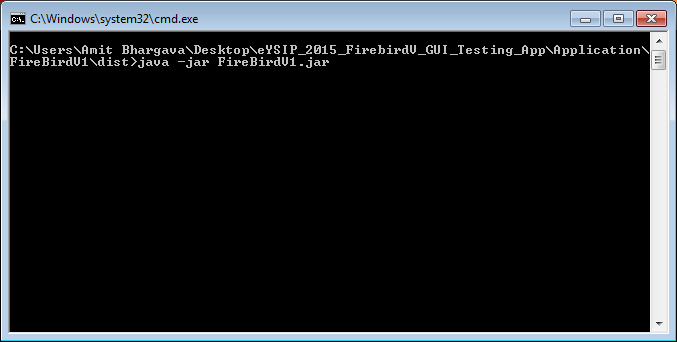
\includegraphics[scale=0.5]{cmd.png}
			\end{center}
		\end{figure}
		After running the command in the command prompt a GUI window will open.
		\item The GUI window will look like this:
		\begin{figure}[h]
			\begin{center}
				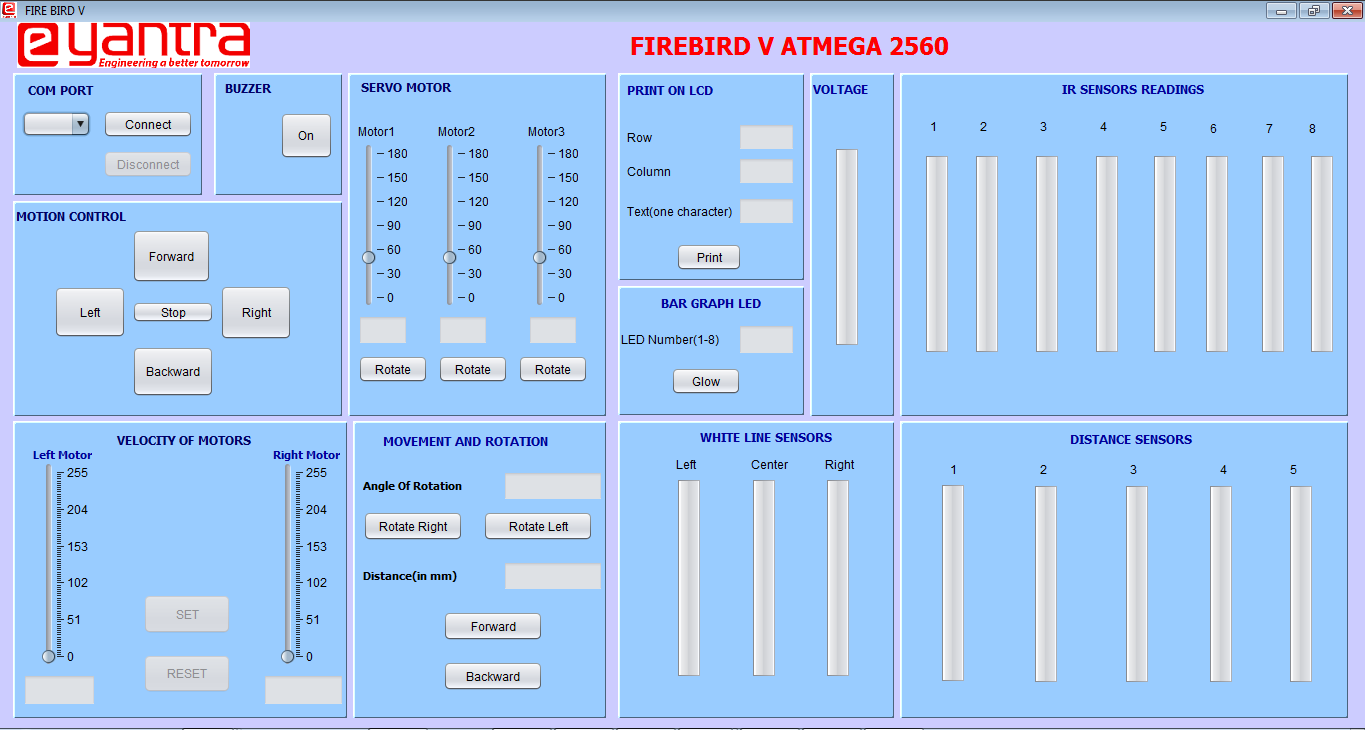
\includegraphics[scale=0.5]{GUI.png}
			\end{center}
		\end{figure} 
		\newpage 
		\item This is a GUI to test various components of Firebird V robot. So the various sections in this GUI tests all the components of Firebird V.
		\item Firstly connect to the Firbird V robot by selecting the COM port in COM PORT section of GUI. Make sure the port in device manager is the COM port of the Firebird V robot. After selecting the COM port click on the connect button to make the connection to the bot. \\
		\begin{figure}[h]
			\begin{center}
				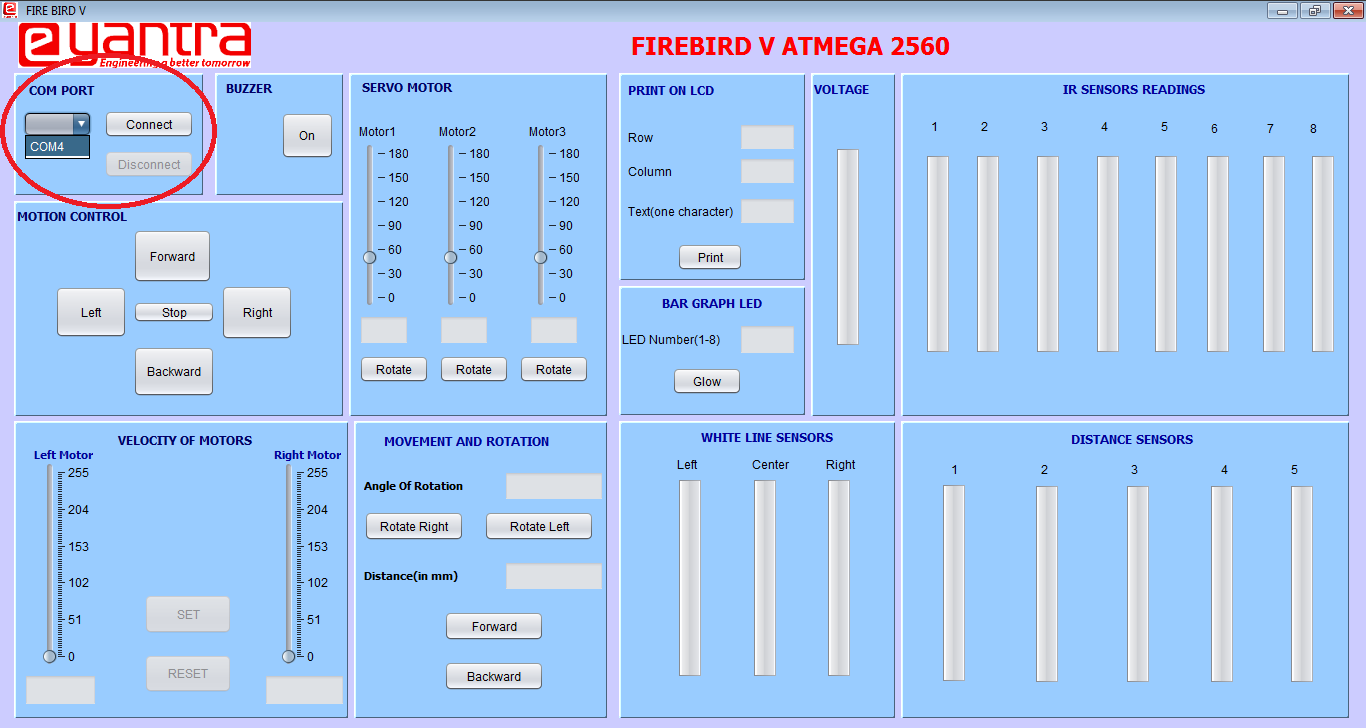
\includegraphics[scale=0.4]{comport.png}
			\end{center}
		\end{figure} 
		\item After connecting to the bot use all the sections of the GUI to test the Firebird V robot.
		\newpage
		\item \textbf{BUZZER SECTION:}\\
		\begin{figure}[h]
			\begin{center}
				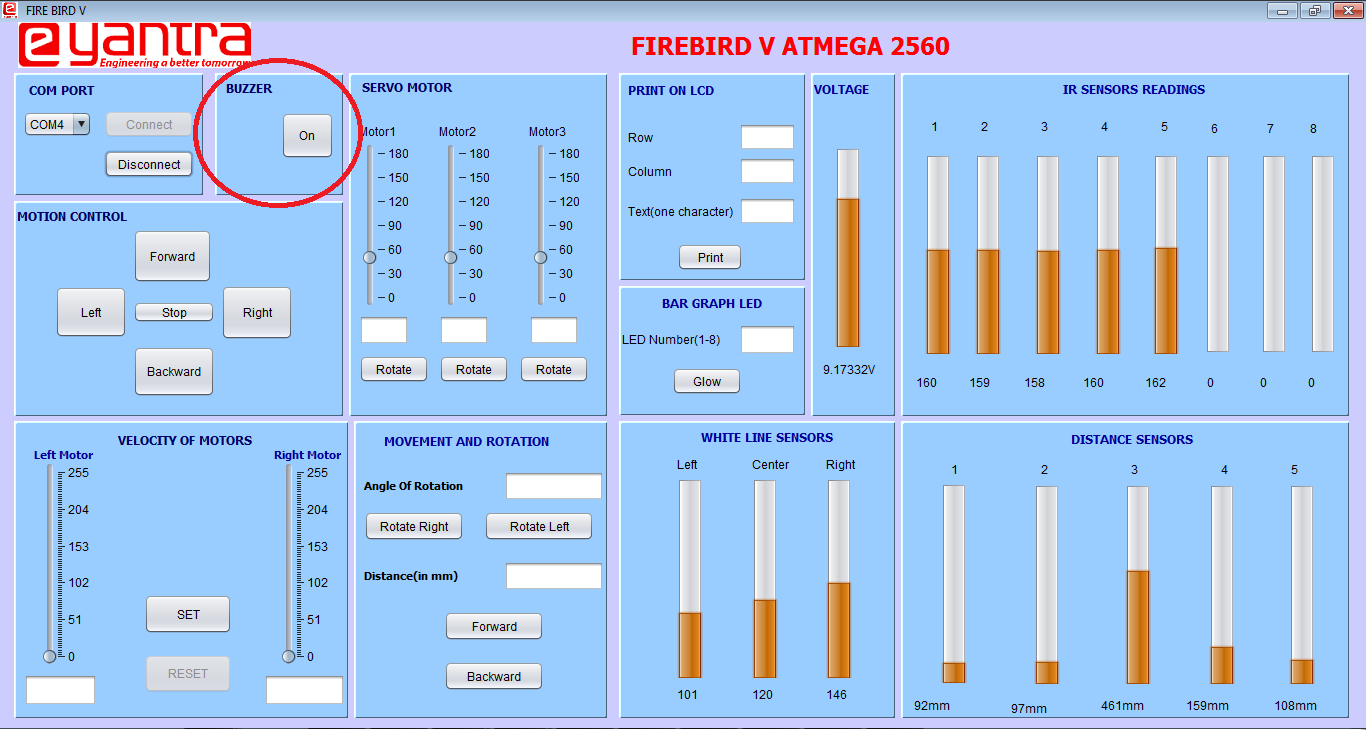
\includegraphics[scale=0.4]{buzzer.png}
			\end{center}
		\end{figure} 
		Click on the button to turn on the buzzer and the buzzer beeps till the user turns off the buzzer by clicking on the button.
		\item \textbf{MOTION CONTROL SECTION:} \\
		\begin{figure}[h]
			\begin{center}
				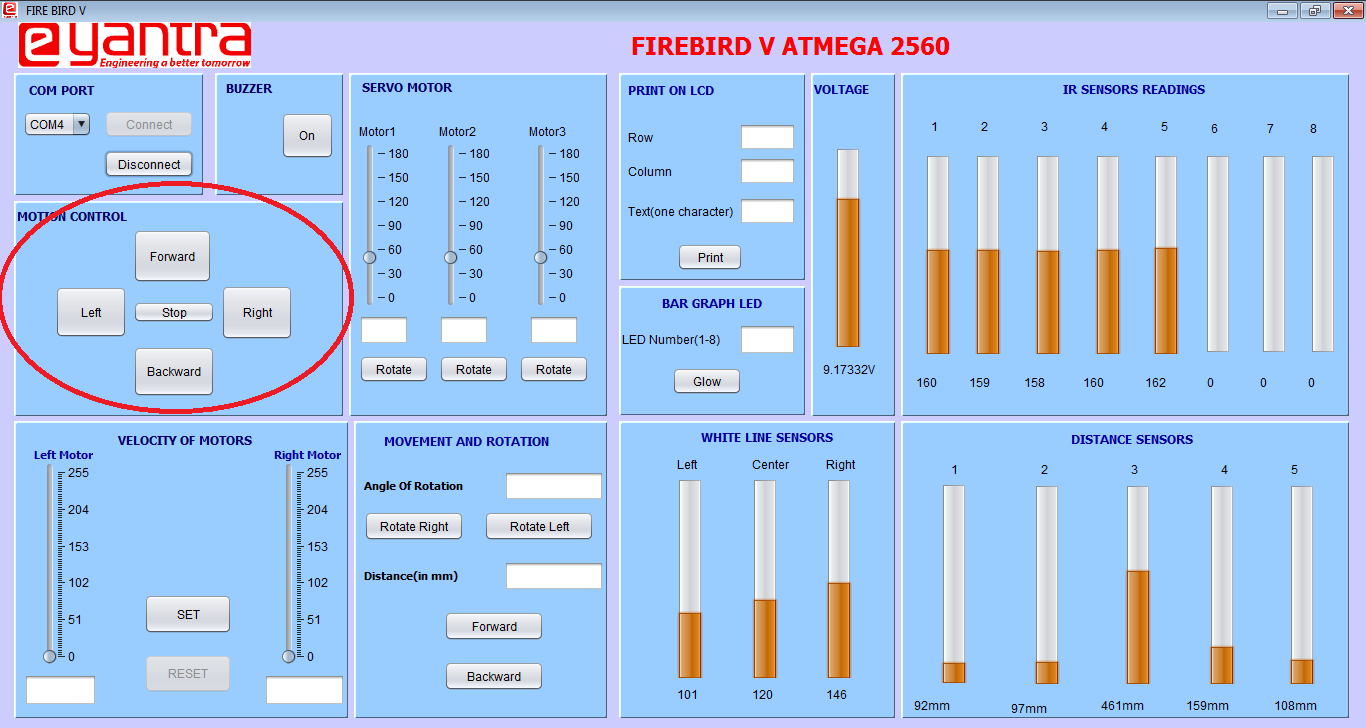
\includegraphics[scale=0.4]{motioncontrol.png}
			\end{center}
		\end{figure}
		This section is used to control the forward, backward, right, left and stop motion of the bot using the buttons.
		\newpage 
		\item \textbf{VELOCITY CONTROL SECTION:} \\
		\begin{figure}[h]
			\begin{center}
				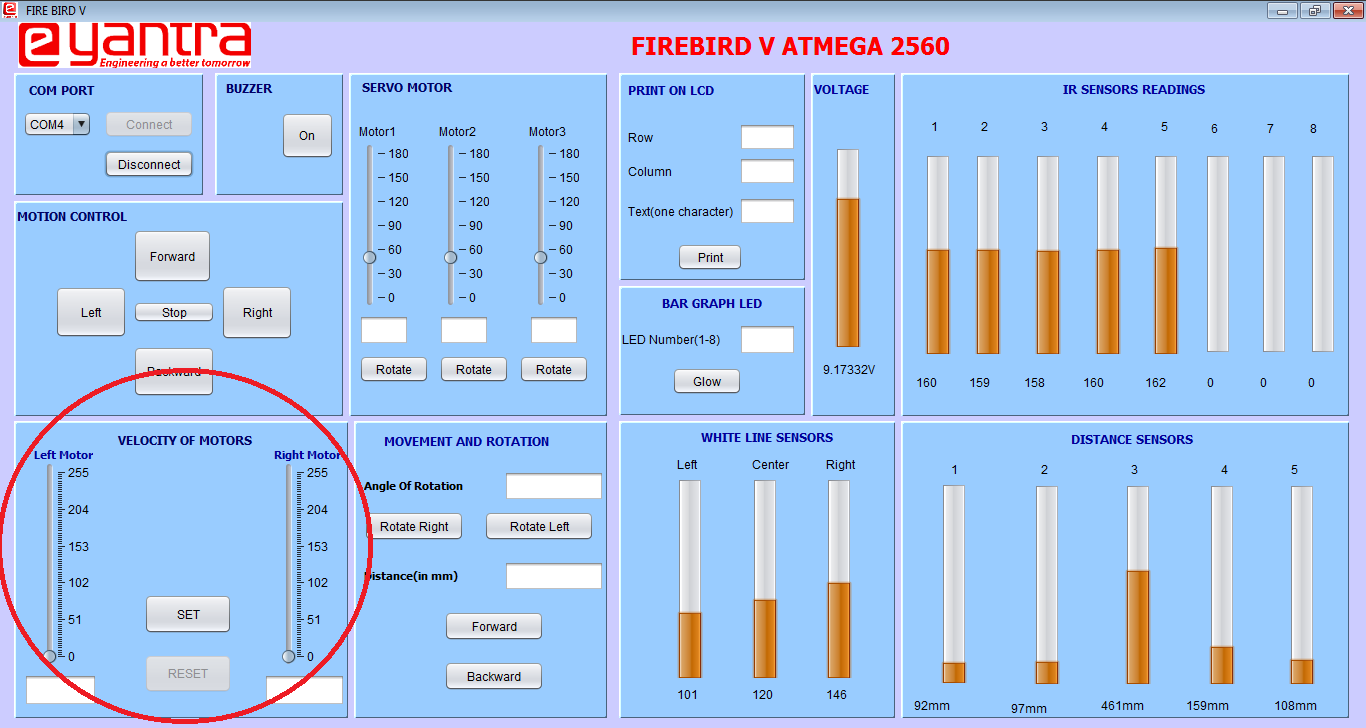
\includegraphics[scale=0.4]{velocitycontrol.png}
			\end{center}
		\end{figure}
		This section is used to control the velocity of left and right motor. Set velocity using the slider or write in the text field and velocity can vary from 0 to 255. After setting the values click on the Set button a message would be seen that the velocity of both motors have been set. Now the motion will be controlled by the velocity set by the user. On clicking the Reset button velocity of both the motors will be set to initial value i.e 255.
		\item \textbf{SERVO MOTOR SECTION:} \\
		\begin{figure}[h]
			\begin{center}
				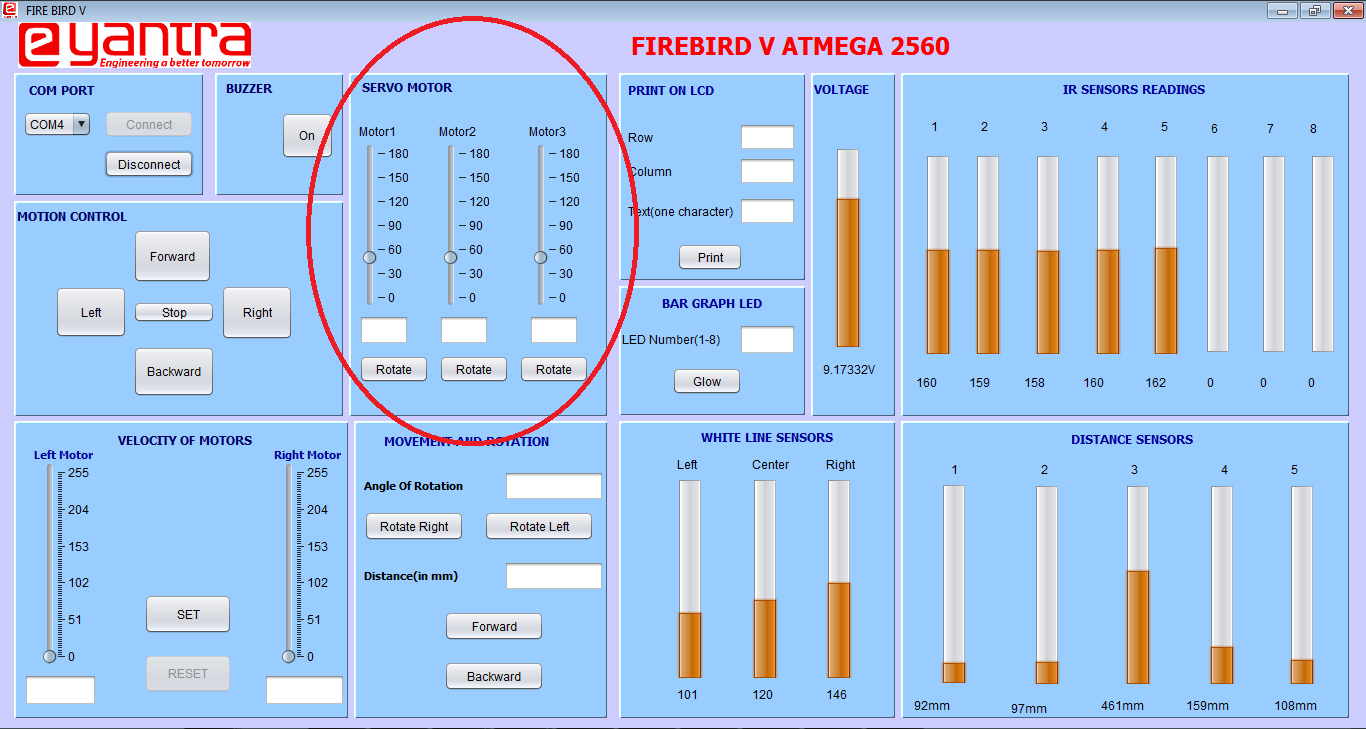
\includegraphics[scale=0.4]{servomotor.png}
			\end{center}
		\end{figure} 
		This section is used to test the servo motors. Set the angle using slider or text field to rotate servo motor by that angle. User ca set the angle from 0 to 180 degrees as servo motor can rotate from 0 to 180 degrees.
		\newpage
		\item \textbf{MOVEMENT AND ROTATION SECTION:} \\
		\begin{figure}[h]
			\begin{center}
				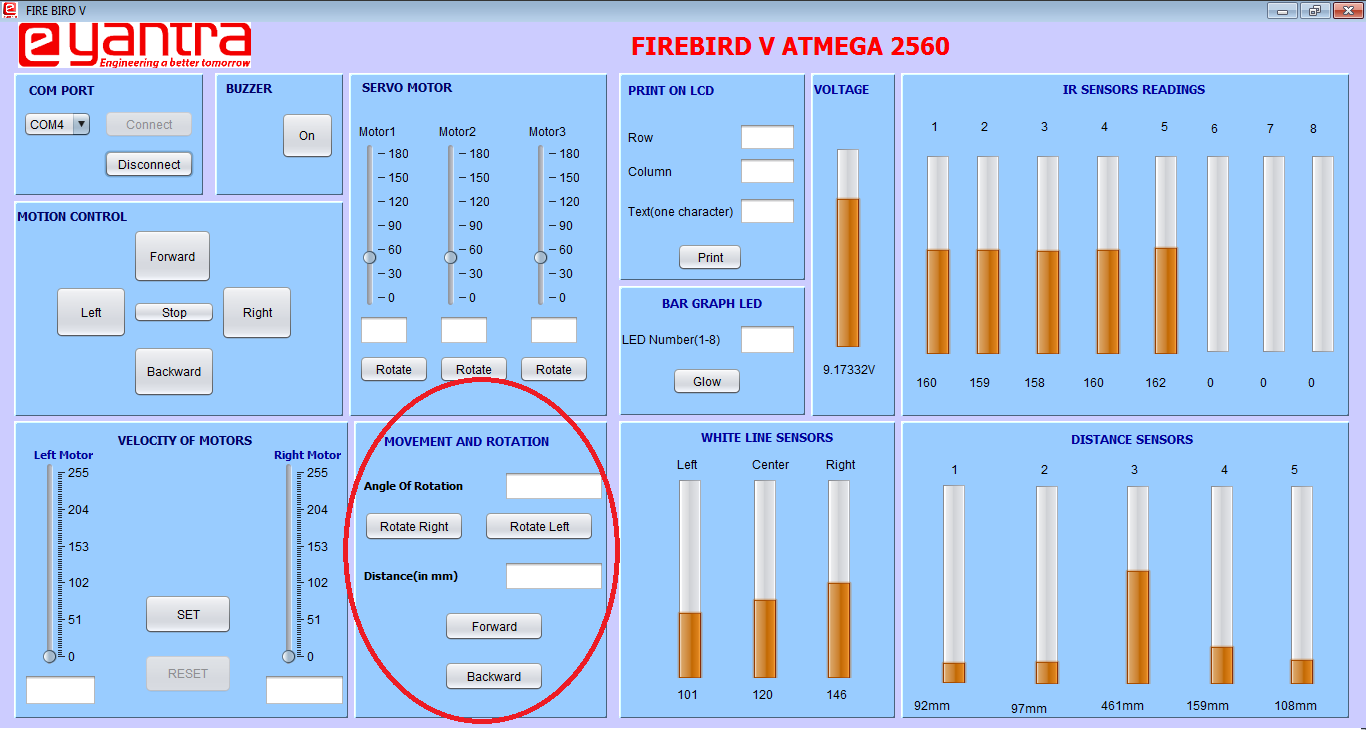
\includegraphics[scale=0.4]{movement_rotation.png}
			\end{center}
		\end{figure}
		This section of GUI checks the position encoders. Rotate the robot left and right by specified angle giving the value of angle in text field. Also move the forward and backward by specified distance by giving distance in millimeter in text field.
		\item \textbf{PRINT ON LCD SECTION:} \\
		\begin{figure}[h]
			\begin{center}
				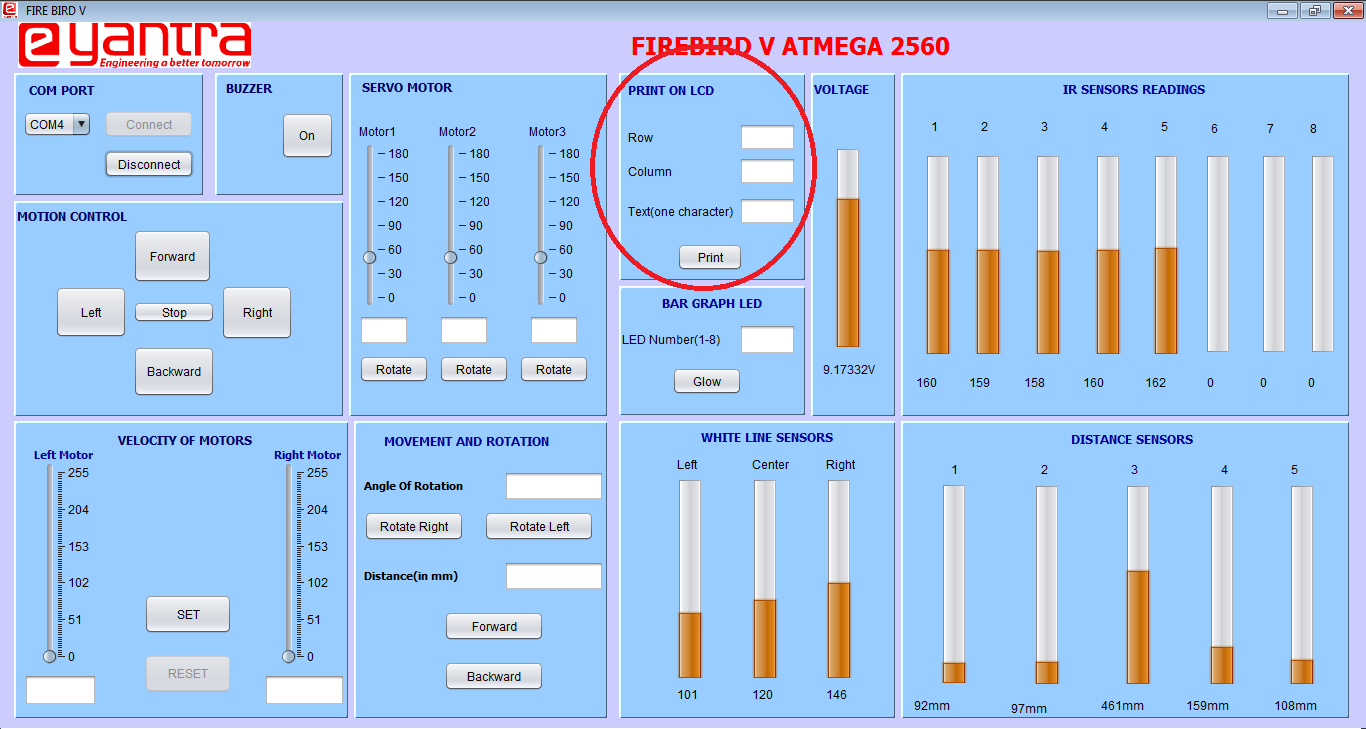
\includegraphics[scale=0.4]{printLCD.png}
			\end{center}
		\end{figure}
		This section prints one character on LCD. Enter the row, column and character to be printed in the text box and click on print button. This will print the character on the specified row and column. The LCD has two rows and 16 columns so user can enter rows from 1 to 2 and column from 1 to 16.
		\newpage
		\item \textbf{BAR GRAPH LED SECTION:} \\
		\begin{figure}[h]
			\begin{center}
				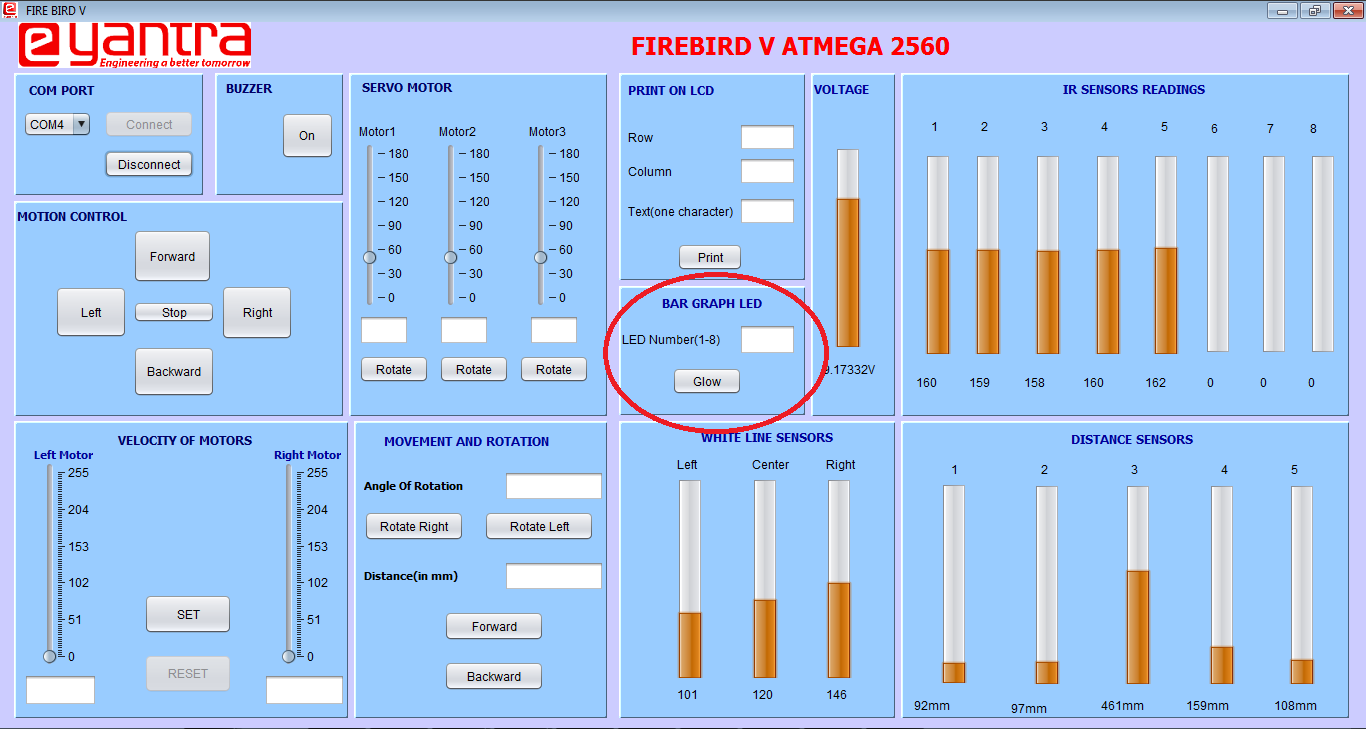
\includegraphics[scale=0.4]{BarLED.png}
			\end{center}
		\end{figure}
		This section is used to test the Bar Graph LED of the Firebird V robot. Enter the LED number to test in the text box and click on Glow button. It will glow the respective LED for 2 seconds. LED 8 is the top most LED and as we move down LED number decreases upto 1.
		\item \textbf{BATTERY VOLTAGE SECTION:} \\
		\begin{figure}[h]
			\begin{center}
				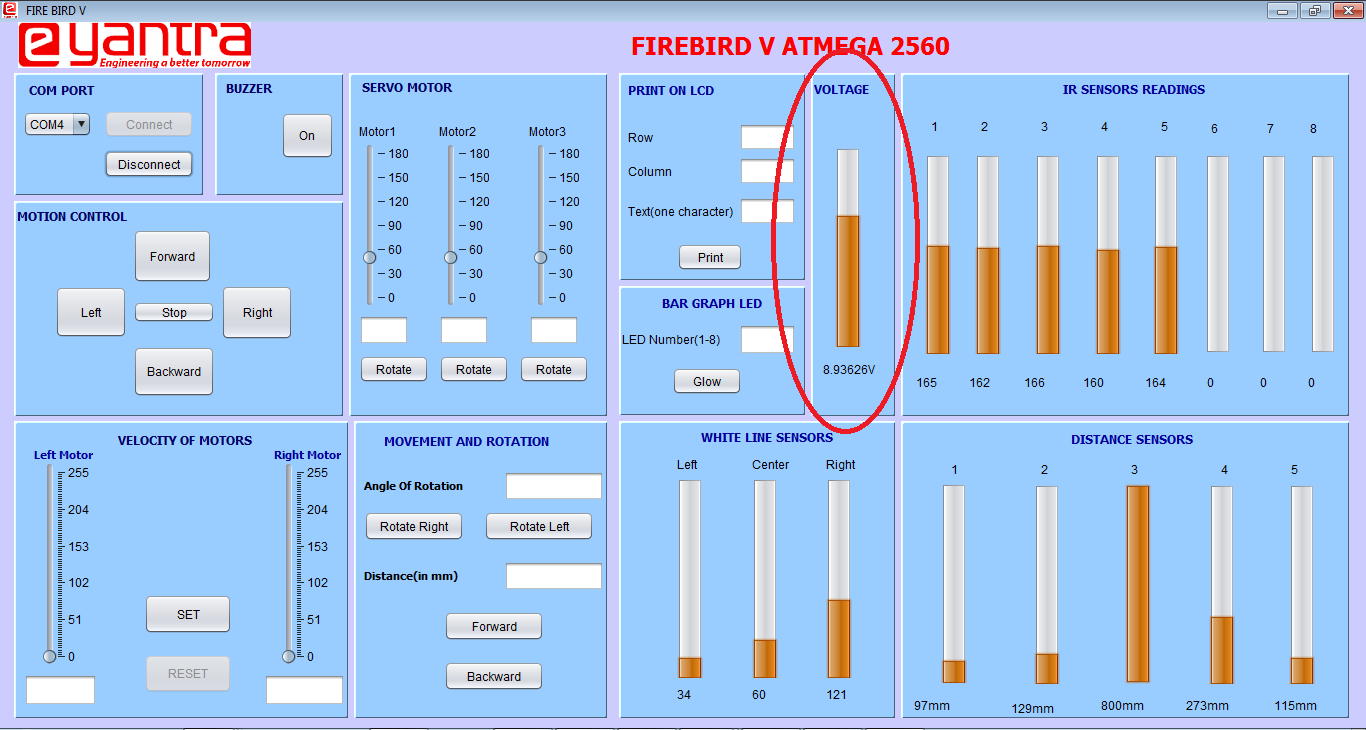
\includegraphics[scale=0.4]{batteryvoltage.png}
			\end{center}
		\end{figure}
		This section gives the reading of battery voltage. Its maximum value is 12V. 
		\newpage
		\item \textbf{WHITE LINE SENSORS SECTION:} \\
		\begin{figure}[h]
			\begin{center}
				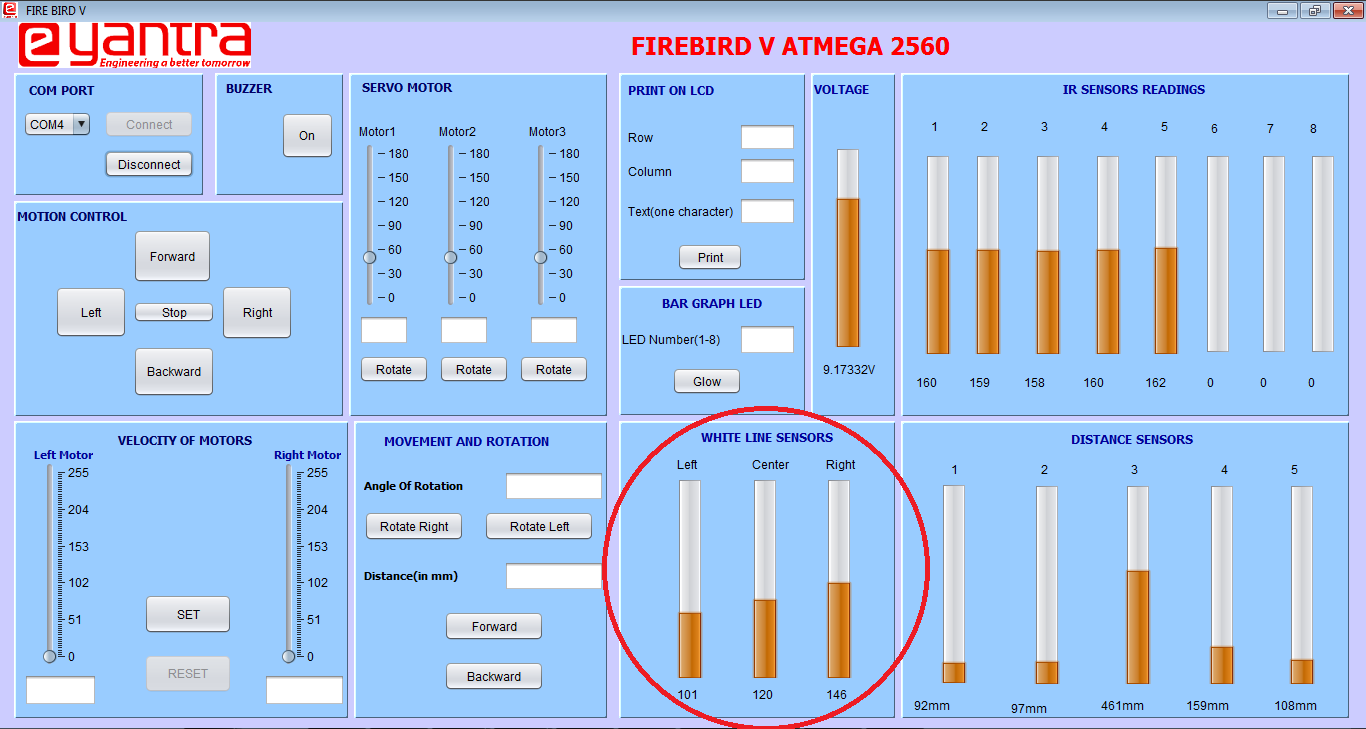
\includegraphics[scale=0.4]{WLSensor.png}
			\end{center}
		\end{figure}
		This section tests the white line sensors. It gives the value of left, center and right white line sensor. It can be used for to decide threshold value for line following. The lower readings are for white surface and higher readings are for black surface. 
		\item \textbf{IR SENSORS SECTION:} \\
		\begin{figure}[h]
			\begin{center}
				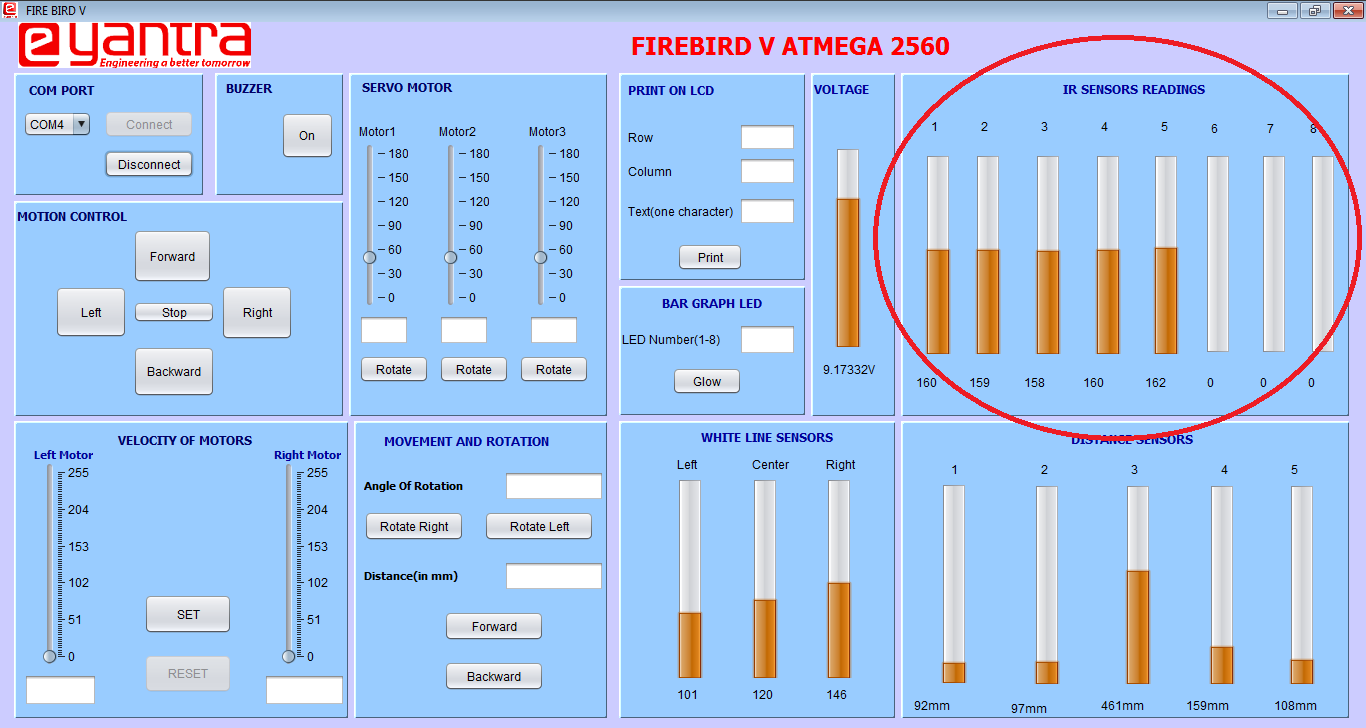
\includegraphics[scale=0.4]{IRSensor.png}
			\end{center}
		\end{figure}
		This section gives the reading of IR Sensors. IR Sensors 6, 7 and 8 works only when jumper 4 is connected. The readings of IR sensors vary from 0 to 255. 
		\newpage
		\item \textbf{DISTANCE SENSORS SECTION:} \\
		\begin{figure}[h]
			\begin{center}
				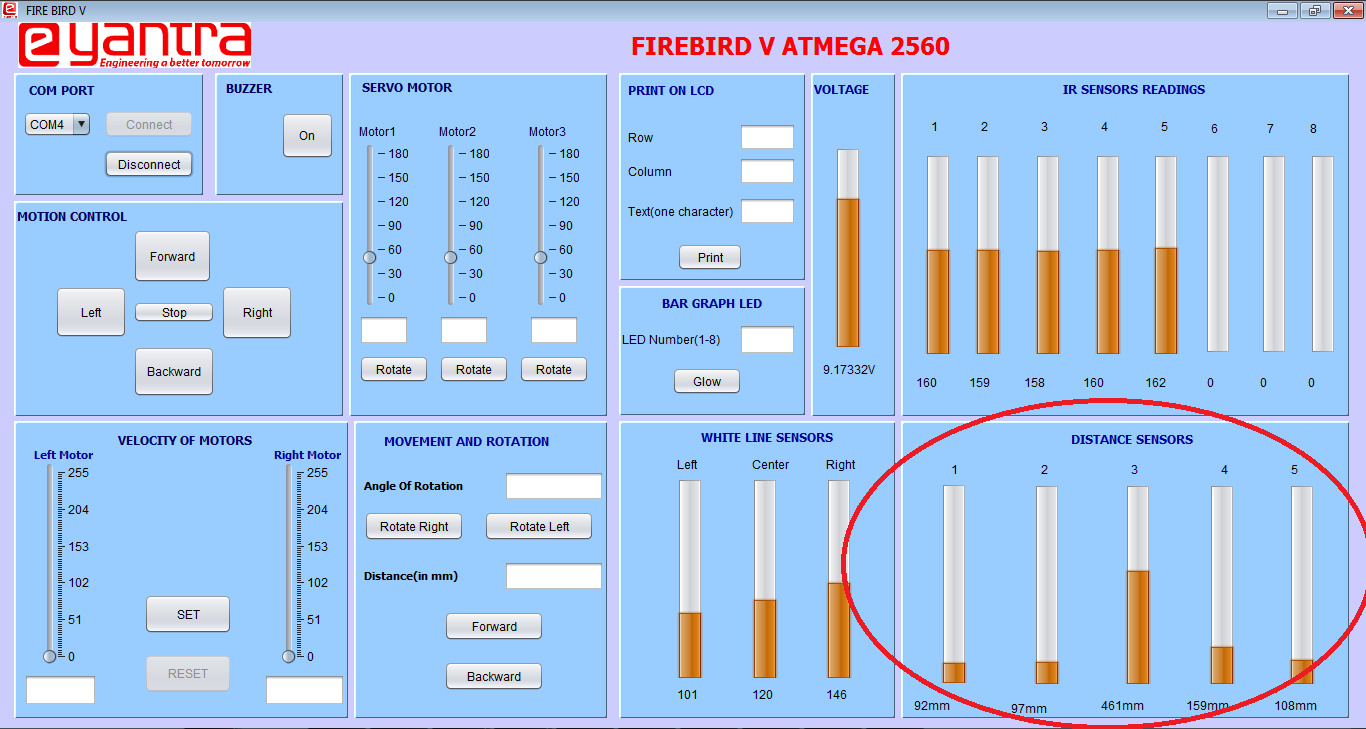
\includegraphics[scale=0.4]{distancesensor.png}
			\end{center}
		\end{figure}
		This section gives the reading of the Distance sensor connected. The distance which is connected gives the correct reading all the other readings are garbage value. The readings of distance sensors vary from 0 mm to 800 mm.
		\item After testing all the components of the Firebird V robot click on the disconnect button to close the connection.
		\begin{figure}[h]
			\begin{center}
				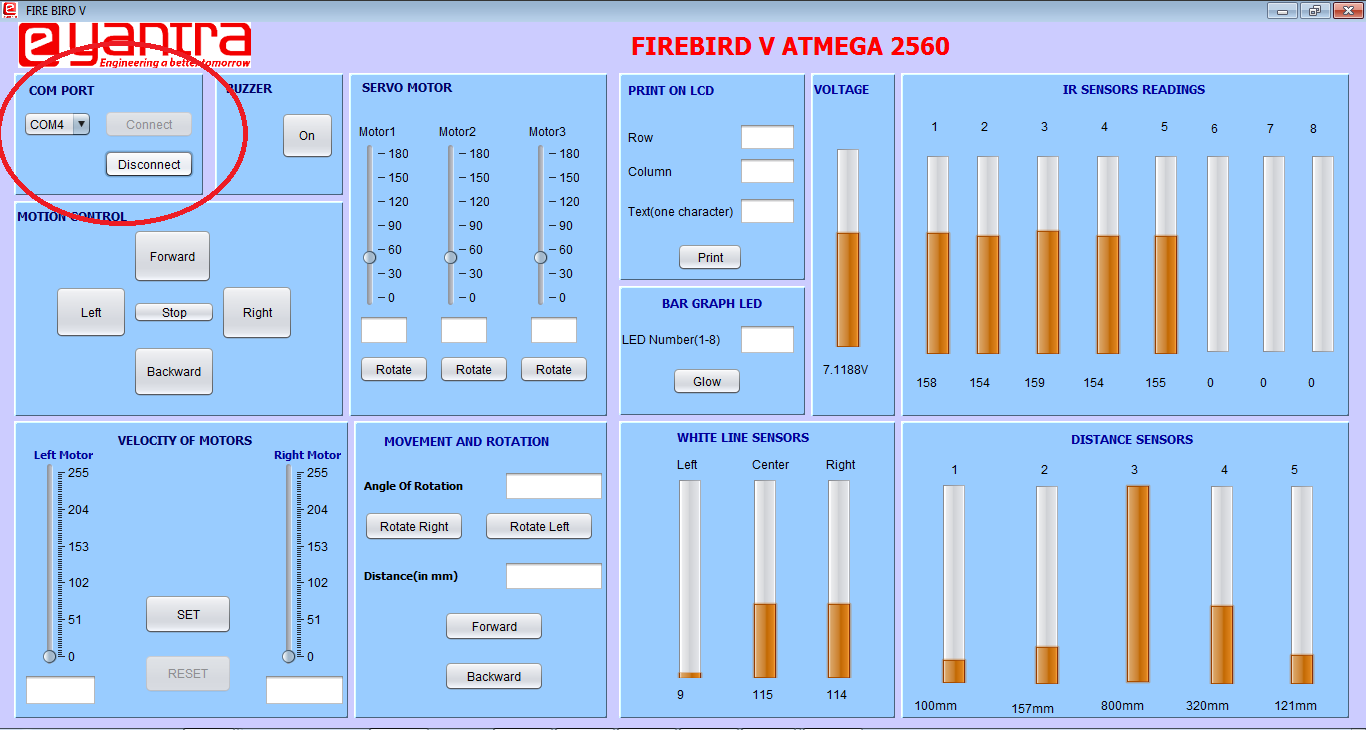
\includegraphics[scale=0.4]{disconnect.png}
			\end{center}
		\end{figure}  
	\end{enumerate}
		
\end{document}